\documentclass[11pt,dvipdfmx]{jarticle}


\oddsidemargin 0cm
\evensidemargin 0cm
\textwidth 16cm
\textheight 24cm
\topmargin -2.0cm
\usepackage[dvipdfmx]{graphicx}
\usepackage{amssymb,amsmath}
\usepackage{color}
\usepackage{fancybox}
\usepackage{ascmac}
\usepackage{amsthm}
\usepackage{url}
\usepackage[normalem]{ulem}

 % 環境次第では, 以下の二つを入れているとエラーが起こる場合があるようです. 
 % コンパイル出来ない場合は, 以下二行をコメントアウト(頭に % を付けると, その行は無視されるようになっています)してみて下さい. 
\usepackage[dvipdfmx]{hyperref}
\usepackage{pxjahyper}

\theoremstyle{definition}
\newtheorem{theorem}{定理}
\newtheorem{definition}{定義}
\newtheorem{proposition}{命題}
\newtheorem{remark}{注意}
\newtheorem{prob}{問}

\newcommand{\Rd}{\partial}
\newcommand{\Rmd}{\mathrm{d}}
\newcommand{\EP}{\varepsilon}

\begin{document}

\begin{center}
\vspace*{6mm}
{\Large 計数工学実験 (統計手法) レポート\\ \vspace*{2mm} Rによる多変量データ解析\\ \vspace*{2mm} --- グラフィカルモデリング ---}\\
\vspace*{4mm}
学籍番号 XX-XXXXXX\\
氏名: 佐藤 瞭
\end{center}

\begin{abstract}
アメリカ合衆国の州ごとの人口やペット(犬・猫)のデータについて,基本統計量や相関行列などを求めた.また,3つ以上の変数の関連を視覚的に捉える為に,共分散選択アルゴリズムを用いたグラフィカルモデリングとして,データに対応した無向独立グラフを導出した.得られた結果に基づいて,データの背景を考察した.
\end{abstract}


\section{データ解析の目的} \label{section:mokuteki}
ペットを飼っている人は,ペットとして飼う動物を選択するときに,どのような要因に影響されているか知りたい,という問題がある.具体的には,犬を飼っている人の割合が高い地域には,人口や面積にどのような特徴があるか知りたい,といった例が挙げられる.今回は, アメリカ合衆国の州ごとに,犬や猫を飼っている人の割合と人口・面積・人口密度の関連を, フリーの統計解析ソフト「R」を用いて解析する.  

2つの変数の関係については,相関を求めることでその傾向を知ることができる. しかし, 3つ以上の変数の傾向をとらえるには,それぞれの相関を見るだけ不十分である. 例えば,人口密度の値を固定したときに,犬を飼っている人の割合と猫を飼っている人の割合の相関がどのようになるかはわからない. 3つ以上の変数の「絡み」をとらえるために,今回は共分散選択アルゴリズムによるグラフィカルモデリングを用いる. これにより,それぞれの変数の「絡み」を無向独立グラフに表し,視覚的にとらえることができる.

基本統計量や相関行列, グラフィカルモデリングで得られた結果をもとに, それぞれから読み取れることの違いに留意しながら, 各変数の関連を探る. 


\section{データ解析} \label{section:gaiyou}
アメリカ合衆国で,ペットとして,淡水魚に次いで最も多く飼われている\cite{number_of_pets}動物である犬と猫のデータと,州ごとの人口・人口密度・面積のデータを解析する.

犬と猫のデータはdata.world\cite{data_world}から取得した.人口などのデータはWorld Population Review\cite{world_population_review}から取得した.2つのテーブルを地名で結合し,アラスカとハワイを除く48の州,及びワシントンD.C.のデータを得た.
データの変数は7個, データ数は49行である.

変数名,変数の説明,表記の簡便さのための変数名の略記を表\ref{table:arribute-info}に記す.

\begin{table}[htbp]
    \caption{変数名の略記,変数名,変数の説明}
    \label{table:arribute-info}
    \begin{center}
        {\small
        \begin{tabular}{|c|ll|}
            \hline
            略記 & \multicolumn{1}{c}{変数名} & \multicolumn{1}{c|}{説明} \\ \hline
            S1 & Density                 & 人口密度 (人 / 平方マイル)        \\
            S2 & Pop\_2019               & 人口 (人,2019年)              \\
            S3 & Area                    & 面積 (平方マイル)              \\
            S4 & Dog.Owners.percentage   & 犬を飼っている人の割合 (%)           \\
            S5 & Mean.Dogs.per.household & 犬を飼っている世帯での犬の平均頭数       \\
            S6 & Cat.Owners.percentage   & 猫を飼っている人の割合 (%)         \\
            S7 & Mean.Cats.per.household & 猫を飼っている世帯での猫の平均頭数       \\ \hline
        \end{tabular}
    }
    \end{center}
\end{table}


\subsection{基本統計量}
データに関して,Rの関数 {\tt summary} を利用して得た要約統計量を表\ref{table:summary}にまとめた.

\begin{table}[htbp]
    \caption{要約統計量}
    \label{table:summary}
    \begin{center}
        {\small
        \begin{tabular}{|c|rrrrrrr|}
            \hline
            & \multicolumn{1}{c}{S1} & \multicolumn{1}{c}{S2} & \multicolumn{1}{c}{S3} & \multicolumn{1}{c}{S4} & \multicolumn{1}{c}{S5} & \multicolumn{1}{c}{S6} & \multicolumn{1}{c|}{S7} \\ \hline
            Min.    & 6                      & 573720                 & 61     & 13.1 & 1.10 & 11.6 & 1.70 \\
            1st Qu. & 55                     & 1932549                & 35826  & 32.9 & 1.40 & 29.0 & 1.90 \\
            Median  & 108                    & 4682509                & 53625  & 36.6 & 1.60 & 31.3 & 2.00 \\
            Mean    & 438                    & 6650367                & 60303  & 37.0 & 1.59 & 31.6 & 2.04 \\
            3rd Qu. & 230                    & 7530552                & 79627  & 42.5 & 1.70 & 33.8 & 2.20 \\
            Max.    & 11535                  & 39776830               & 261232 & 47.9 & 2.10 & 49.5 & 2.60 \\ \hline
        \end{tabular}
    }
    \end{center}
\end{table}


\subsection{相関行列と対散布図}

成績データの相関行列を表\ref{table:cor}に,偏相関行列を表\ref{table:par}に示す.相関行列と偏相関行列を区別するために,ここでは偏相関行列の対角成分は --- で表すという慣習にしたがう.また,ともに対称行列であるため,右上成分は示していない.


データの対散布図を図\ref{fig:pairs}に示す. 

\begin{table}[htbp]
\caption{データから直接計算した相関行列.}
\label{table:cor}
\begin{center}
{\small
 \begin{tabular}{|c|rrrrrrr|}
  \hline
  & S1 & S2 & S3 & S4 & S5 & S6 & S7 \\
  \hline
  S1	& 1.0000 & & & & & & \\
  S2	& -0.0884 &	1.0000 & & & & & \\
  S3	& -0.2612 &	0.4419 & 1.0000 & & & &\\
  S4	& -0.5962 & -0.0638	& 0.3986 & 1.0000 & & &\\ 
  S5	& -0.4252 &	0.0478 & 0.3911 & 0.7919 & 1.0000 & &\\ 
  S6	& -0.5458 &	-0.2379	& -0.0243 &	0.3767 & 0.1639 & 1.0000 & \\
  S7	& -0.1478 &	0.0154 & 0.1290	& 0.4171 & 0.4534 &	-0.1064 & 1.0000 \\
  \hline
 \end{tabular}
}
\end{center}
\end{table}

\begin{table}[htbp]
    \caption{データから直接計算した偏相関行列.}
    \label{table:par}
    \begin{center}
        {\small
            \begin{tabular}{|c|rrrrrrr|}
                \hline
                & S1 & S2 & S3 & S4 & S5 & S6 & S7 \\
                \hline
                S1	& ------ & & & & & & \\
                S2	& -0.2634 &	------ & & & & & \\
                S3	& 0.0050	& 0.4641 &	------ & & & & \\
                S4	& -0.3346	& -0.2666 &	0.2865 &	------ & & & \\
                S5	& 0.0273	& 0.0788 &	0.0617 &	0.652 &	------ & & \\
                S6	& -0.4594	& -0.2232 & -0.1094 &	0.211 &	-0.1141 &	------ & \\
                S7	& -0.0087	& 0.0169 &	-0.1270 &	0.221 &	0.1706 &	-0.261 &	------ \\
                \hline
            \end{tabular}
        }
    \end{center}
\end{table}

\begin{figure}[htbp]
    \begin{center}
        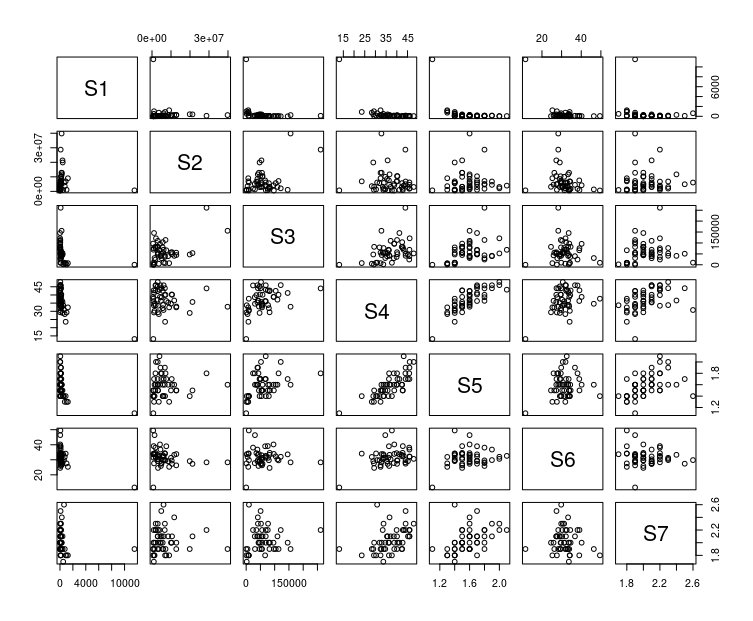
\includegraphics[width=\linewidth]{pairs}
        \caption{データの対散布図.}
        \label{fig:pairs}
    \end{center}
\end{figure}
\clearpage
相関行列,偏相関行列や対散布図からデータに関して分かることとして,たとえば以下のようなことが挙げられる.
\begin{itemize}
    \item 犬を飼っている人の割合と,犬を飼っている世帯での犬の平均頭数には,やや強い正の相関がある.
    \item 相関行列をみると,面積と犬を飼っている世帯での犬の平均頭数には正の相関があるように見えるが,偏相関係数をみるとほとんど相関がないので,他の変数が絡んでいることが予想される.
    \item 面積と犬を飼っている人の割合には弱い正の相関があるが,面積と猫を飼っている人の割合にはほぼ相関がない.
\end{itemize}



\subsection{共分散選択} \label{subsection:sentaku}

成績データに関して, 共分散選択を行なったところ, 28個の偏相関係数のうち11個をゼロとおいたモデルが選択された.選択されたモデルでの相関行列を表~\ref{table:cor-final}に,偏相関行列の推定値を表~\ref{table:par-final}に示す.ゼロとおいた偏相関係数には下線をつけてある,また,除去される辺の順番とAICの変化を表~\ref{table:aic}に示す. さらに, 対応する無向独立グラフを図~\ref{fig:graph-final} に示す. 

\begin{table}[htbp]
\caption{選択されたモデルでの相関行列の推定値. }
\label{table:cor-final}
\begin{center}{\small
    \begin{tabular}{|c|rrrrrrr|}
        \hline
        & \multicolumn{1}{c}{S1} & \multicolumn{1}{c}{S2} & \multicolumn{1}{c}{S3} & \multicolumn{1}{c}{S4} & \multicolumn{1}{c}{S5} & \multicolumn{1}{c}{S6} & \multicolumn{1}{c|}{S7} \\ \hline
        S1 & 1.0000                 &                        &                        &                        &                        &                        &                         \\
        S2 & -0.0884                & 1.0000                 &                        &                        &                        &                        &                         \\
        S3 & -0.2970                & 0.4419                 & 1.0000                 &                        &                        &                        &                         \\
        S4 & -0.5962                & -0.0638                & 0.3986                 & 1.0000                 &                        &                        &                         \\
        S5 & -0.4540                & -0.0395                & 0.3208                 & 0.7919                 & 1.0000                 &                        &                         \\
        S6 & -0.5458                & -0.2379                & 0.0238                 & 0.3160                 & 0.2045                 & 1.0000                 &                         \\
        S7 & -0.1117                & 0.0299                 & 0.1542                 & 0.3270                 & 0.4534                 & -0.1064                & 1.0000                  \\ \hline
    \end{tabular}}
\end{center}
\end{table}

\begin{table}[htbp]
    \caption{選択されたモデルでの偏相関行列の推定値. }
    \label{table:par-final}
    \begin{center}{\small
            \begin{tabular}{|c|rrrrrrr|}
                \hline
                & \multicolumn{1}{c}{S1}     & \multicolumn{1}{c}{S2}     & \multicolumn{1}{c}{S3}     & \multicolumn{1}{c}{S4}     & \multicolumn{1}{c}{S5}     & \multicolumn{1}{c}{S6}     & \multicolumn{1}{c|}{S7}     \\ \hline
                S1 & \multicolumn{1}{c}{------} &                            &                            &                            &                            &                            &                             \\
                S2 & -0.271                     & \multicolumn{1}{c}{------} &                            &                            &                            &                            &                             \\
                S3 &  0                      & 0.482                      & \multicolumn{1}{c}{------} &                            &                            &                            &                             \\
                S4 & -0.363                     & -0.230                     & 0.284                      & \multicolumn{1}{c}{------} &                            &                            &                             \\
                S5 & 0                    &  0                    &  0                      & 0.656                      & \multicolumn{1}{c}{------} &                            &                             \\
                S6 & -0.516                     & -0.300                     &  0                     &  0                    &  0                     & \multicolumn{1}{c}{------} &                             \\
                S7 &  0                     &  0                      &  0               & 0                   & 0.329                      & -0.184                     & \multicolumn{1}{c|}{------} \\ \hline
        \end{tabular}}
    \end{center}
\end{table}



\begin{table}[htbp]
	\caption{除去される辺の順番とAICの変化. }
	\label{table:aic}
	\begin{center}{\small
			\begin{tabular}{|c|rrrrrr|}
                \hline
                反復回数   & \multicolumn{1}{c}{1} & \multicolumn{1}{c}{2} & \multicolumn{1}{c}{3} & \multicolumn{1}{c}{4} & \multicolumn{1}{c}{5} & \multicolumn{1}{c|}{6}  \\ \hline
                除去される辺 & (S3, S1)              & (S7, S1)              & (S7, S2)              & (S5, S1)              & (S5, S3)              & (S5, S2)               \\
                AIC    & -2.00                 & -3.99                 & -5.98                 & -7.94                 & -9.76                 & -11.02                 \\
                AICの変化 & ------ & -1.99 & -1.99 & -1.96 & -1.82 & -1.26 \\ \hline
            \end{tabular}
            \\ \vspace{3mm}
            \begin{tabular}{|c|rrrrr|}
                \hline
                反復回数   & \multicolumn{1}{c}{7} & \multicolumn{1}{c}{8} & \multicolumn{1}{c}{9} & \multicolumn{1}{c}{10} & \multicolumn{1}{c|}{11} \\ \hline
                除去される辺 & (S7, S3)              & (S6, S3)              & (S6, S5)              & (S6, S4)               & (S7, S4)                        \\
                AIC    & -12.35                & -13.81                & -14.17                & -15.14                 & -15.67              \\ 
                AICの変化 & -1.33 & -1.46 & -0.36 & -0.97 & -0.53 \\ \hline
        \end{tabular}}
	\end{center}
\end{table}

\begin{figure}[htbp]
    \begin{center}
        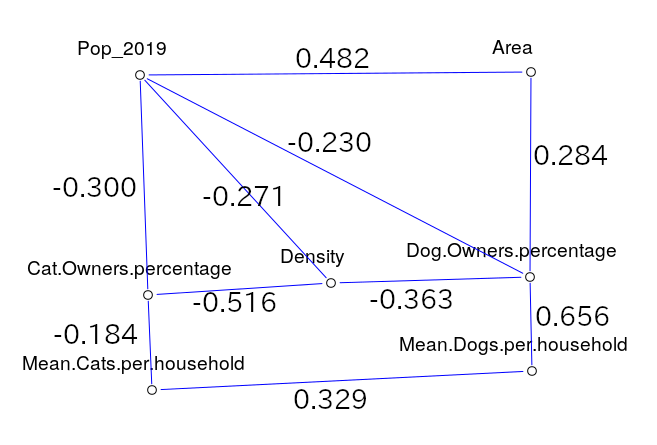
\includegraphics[width=\linewidth]{graph_num}
        \caption{成績データの無向独立グラフ (辺の上の数字は偏相関係数である) .}
        \label{fig:graph-final}
    \end{center}
\end{figure}
\clearpage



\section{考察}
まずは,グラフィカルモデリングに対応した無向独立グラフ(図~\ref{fig:graph-final})からわかることを考察する.任意の2頂点について,2つを結ぶときに必ず通らなければならない点は存在しないため,分離定理を適用できるような頂点集合の組は存在しないことがわかる.そのため,この無向独立グラフからは,条件付き独立な変数の組は見つからない.そのため,人口・人口密度・面積といった情報のうち,犬や猫のうちどちらか一方の所有率や所有数に影響する変数はないことがわかる.

ここで,猫に関する変数と,犬に関する変数の,グラフ上での違いを2点に絞って考える.
\begin{enumerate}
    \item まず,(猫の所有率,面積)の辺は除去されているのに対して,(犬の所有率,面積)の辺は除去されていない点が挙げられる.実際に犬や猫を飼う場面を思い浮かべてみると,犬を飼う場合は,ドッグランのような屋外の開けた場所で遊ばせる場面が想定でき,ある程度広い土地がある地域のほうが犬を遊ばせやすいことが考えられる.実際,(犬の所有率,面積)の偏相関係数は正の値になっていることから,土地が広い地域では犬を飼うことに対して積極的であるのではないか,という仮説を立てることができる.一方で,猫を飼う場合は,家の中で飼ってあまり外に出さないようなケースが犬よりも多い(日本の調査\cite{pet_survey}ではこのような傾向がみられる)ために,犬の場合ほど広い土地を必要としない,という説明が考えられる.
    \item つぎに,(猫の所有率,猫を飼っている世帯での猫の平均頭数)には偏相関がほぼないのに加えて偏相関係数が負になっているのに対して,(犬の所有率,犬を飼っている世帯での犬の平均頭数)にはやや強い正の偏相関がある点が挙げられる.犬を飼っている世帯が多い地域では犬を飼っている頭数が多くなる傾向にあるが,猫ではこのような傾向がみられない背景として,飼い主同士の接触の機会の多寡が影響している可能性が考えられる.犬を飼っている場合は散歩などで外に出る機会がある.その際に,犬の所有率が高い地域であれば他の飼い主と遭遇する確率も高くなる.一方,猫を飼っている場合は,家の中で飼っていてあまり外に連れ出さない場合が犬よりも多く\cite{pet_survey},飼い主同士の接触の機会は,犬の場合と比べて少ないと予想される.仮に,飼い主同士の接触が多いと,飼い主はより多くのペットを飼いたくなる,という傾向があるとすれば,今回発見した傾向の説明はつく.飼い主同士の接触の多寡とペットを飼っている頭数の関係を新たに調べることで,この仮説は検証できるだろう.
\end{enumerate}

他の特徴的な点として,(猫を飼っている世帯での猫の平均頭数,犬を飼っている世帯での犬の平均頭数)の辺がグラフに残っており,この辺が残っているために,この変数対が条件付独立でなくなっている点が挙げられる.偏相関係数をみると0.329となっており,弱い正の偏相関があることが確認できる.この背景として,動物の種類に限らず,周囲にペットの所有者が多いと自分も飼いたくなる,といった同調効果の可能性が挙げられるほか,ペットの所有率が高い地域はペットを飼い始める障壁が低い環境(たとえば,予防接種や去勢の費用を自治体が負担してくれる,といった金銭面の環境)にある,といった仮説が考えられる.

つぎに,AICの変化について考察する.まずAICの定義は,
\[
{\rm AIC} = - 2 \times(最大対数尤度) - 2 \times (制約式の個数) + (定数)
\]
であった.つまり,AICはモデルのデータの当てはまりが良いほど,また,グラフの辺が少ないほど大きくなる.また,グラフの辺を1つ減らすたびに,$ - 2 \times (制約式の個数) $の項は$-2$ずつ変化していく.そのため,AICの変化量に2を足した値が,制約を増やすことによって犠牲になった,モデルの当てはまりの良さであると解釈できる.このことを踏まえた上で,表~\ref{table:aic}のAICの変化を見てみる.反復回数が大きくなるにつれて,AICの変化量は概ね小さくなっている.すなわち,反復回数が大きくなるにつれて,制約を増やすために,モデルの当てはまりの良さをより大きく犠牲にしていることが確認できる.
他の除去と比べてAICの変化の大きさが大きい例として,2回目で除去される辺(S7,S1)が挙げられる.この除去によるAICの変化は-1.99であり,この辺はモデルから取り除いても当てはまりの良さはほとんど失われないため,制約を増やすために早い反復回数で除去されたと解釈できる.この辺に対応する変数対は,猫を飼っている世帯での猫の平均頭数と人口密度である.実際,最終的に得た無向独立グラフでは,両者は猫の所有率という変数を間に挟んで結ばれており,猫を飼っている世帯での猫の平均頭数と人口密度の相関は別の変数によるものであったといえる.
\begin{thebibliography}{9}
\bibitem{number_of_pets}
Number of pets in the United States in 2017/2018, by species (in millions),https://www.statista.com/statistics/198095/pets-in-the-united-states-by-type-in-2008/,2019/04/22 閲覧.
\bibitem{data_world}
Cat vs. Dog Popularity in U.S.,https://data.world/datanerd/cat-vs-dog-popularity-in-u-s,2019/04/22 取得.
\bibitem{world_population_review}
US States by Density 2019,http://worldpopulationreview.com/states/state-densities/,2019/04/22 取得.
\bibitem{pet_survey}
平成30年 全国犬猫飼育実態調査「主要指標 サマリー」,ペットフード協会,https://petfood.or.jp/data/chart2018/3.pdf,p.21,2019/04/25 閲覧.
\end{thebibliography}


\end{document}
